\chapter{Injection test for $B^0$ signal yield}

To test the reliability of the signal extraction using 2D fit in the current low statistics of experiment data, an injection test is performed where we inject 5 to 30 signal events with 46 background events randomly taken from the \textit{generic MC}. The distribution of the each test is included in Figure \ref{fig:injectiontest}.
\begin{figure}[htpb]
	\begin{subfigure}{0.5\linewidth}
		\includegraphics[page=1,height=6cm]{figures/injection_sig_5/ds_gen_Mbc_2D.pdf}
		\caption{signal injected: 5}
	\end{subfigure}
	\begin{subfigure}{0.5\linewidth}
		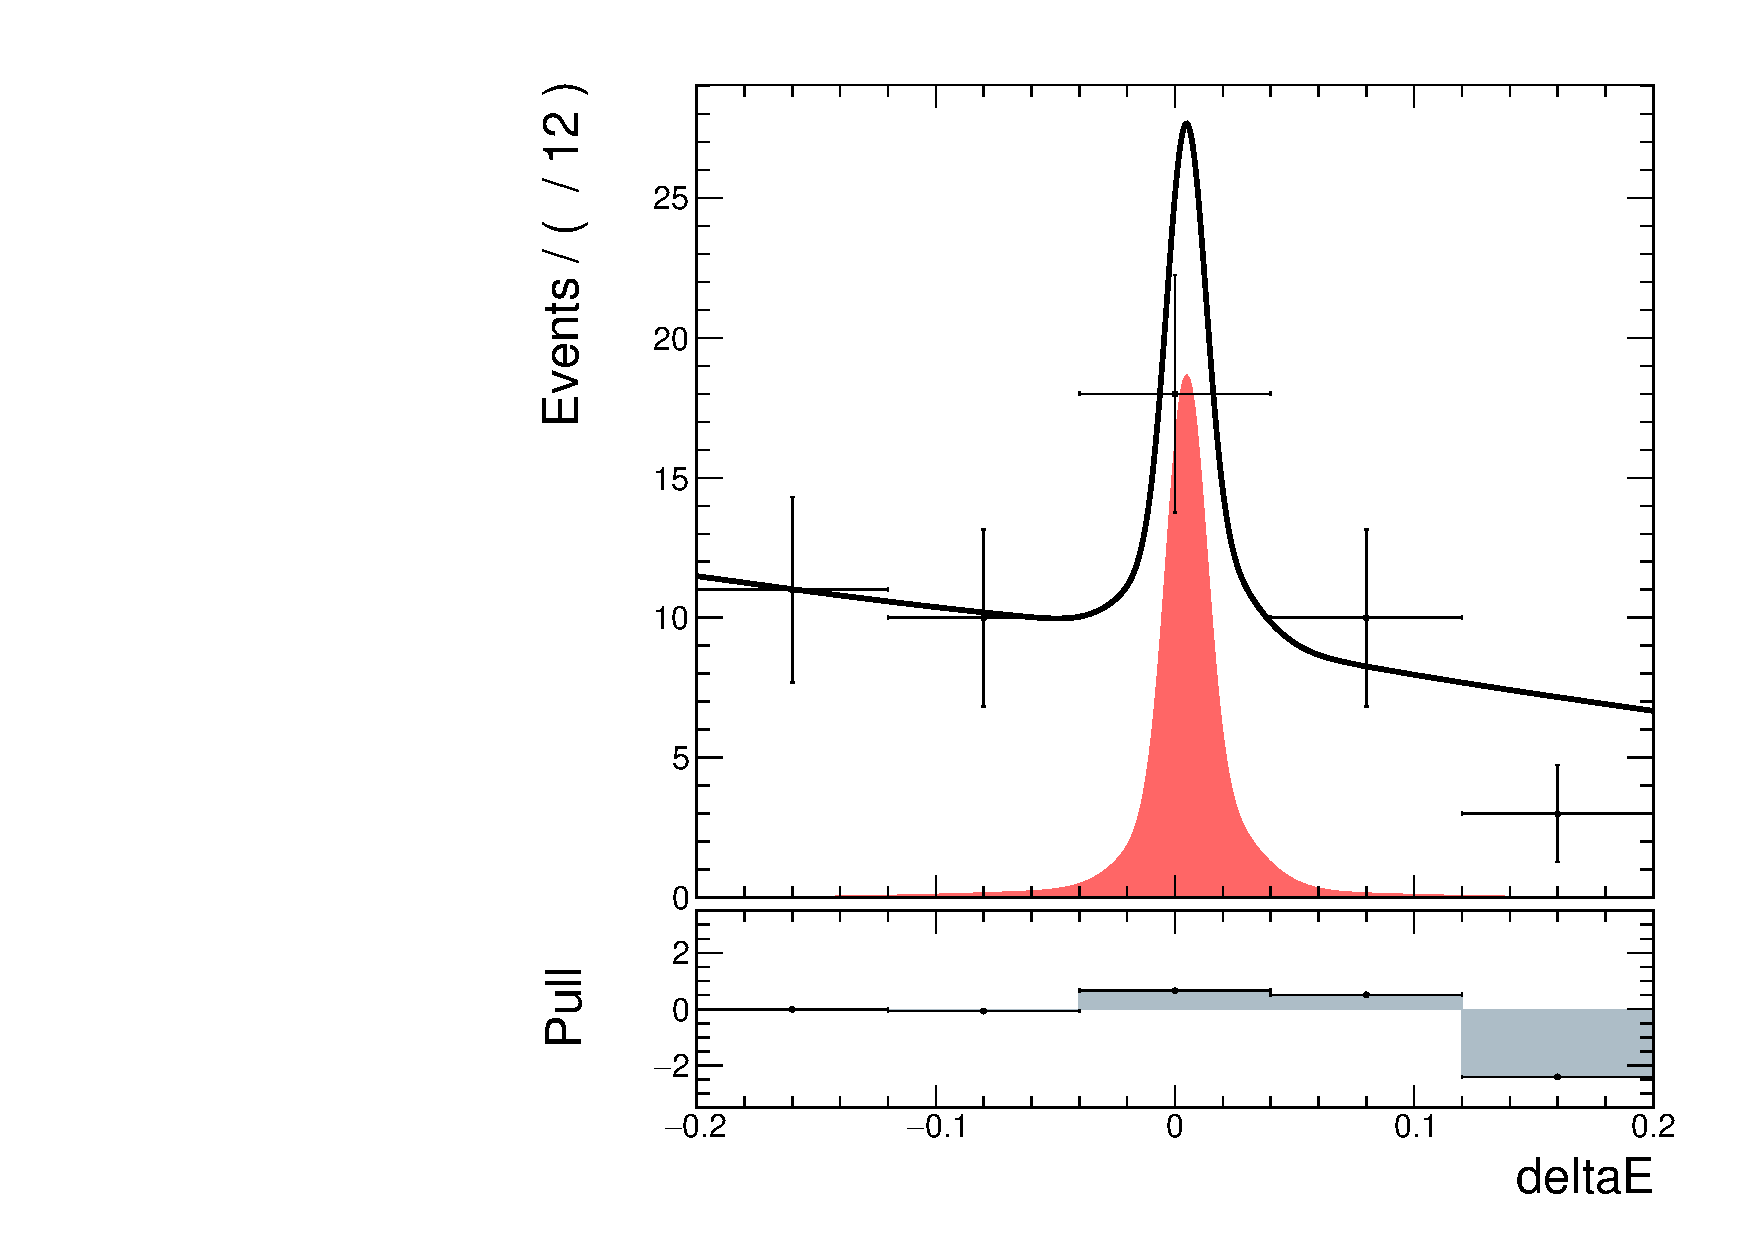
\includegraphics[page=1,height=6cm]{figures/injection_sig_5/ds_gen_deltaE_2D.pdf}
		\caption{signal injected: 5}
	\end{subfigure}
	\begin{subfigure}{0.5\linewidth}
		\includegraphics[page=1,height=6cm]{figures/injection_sig_10/ds_gen_Mbc_2D.pdf}
		\caption{signal injected: 10}
	\end{subfigure}
	\begin{subfigure}{0.5\linewidth}
		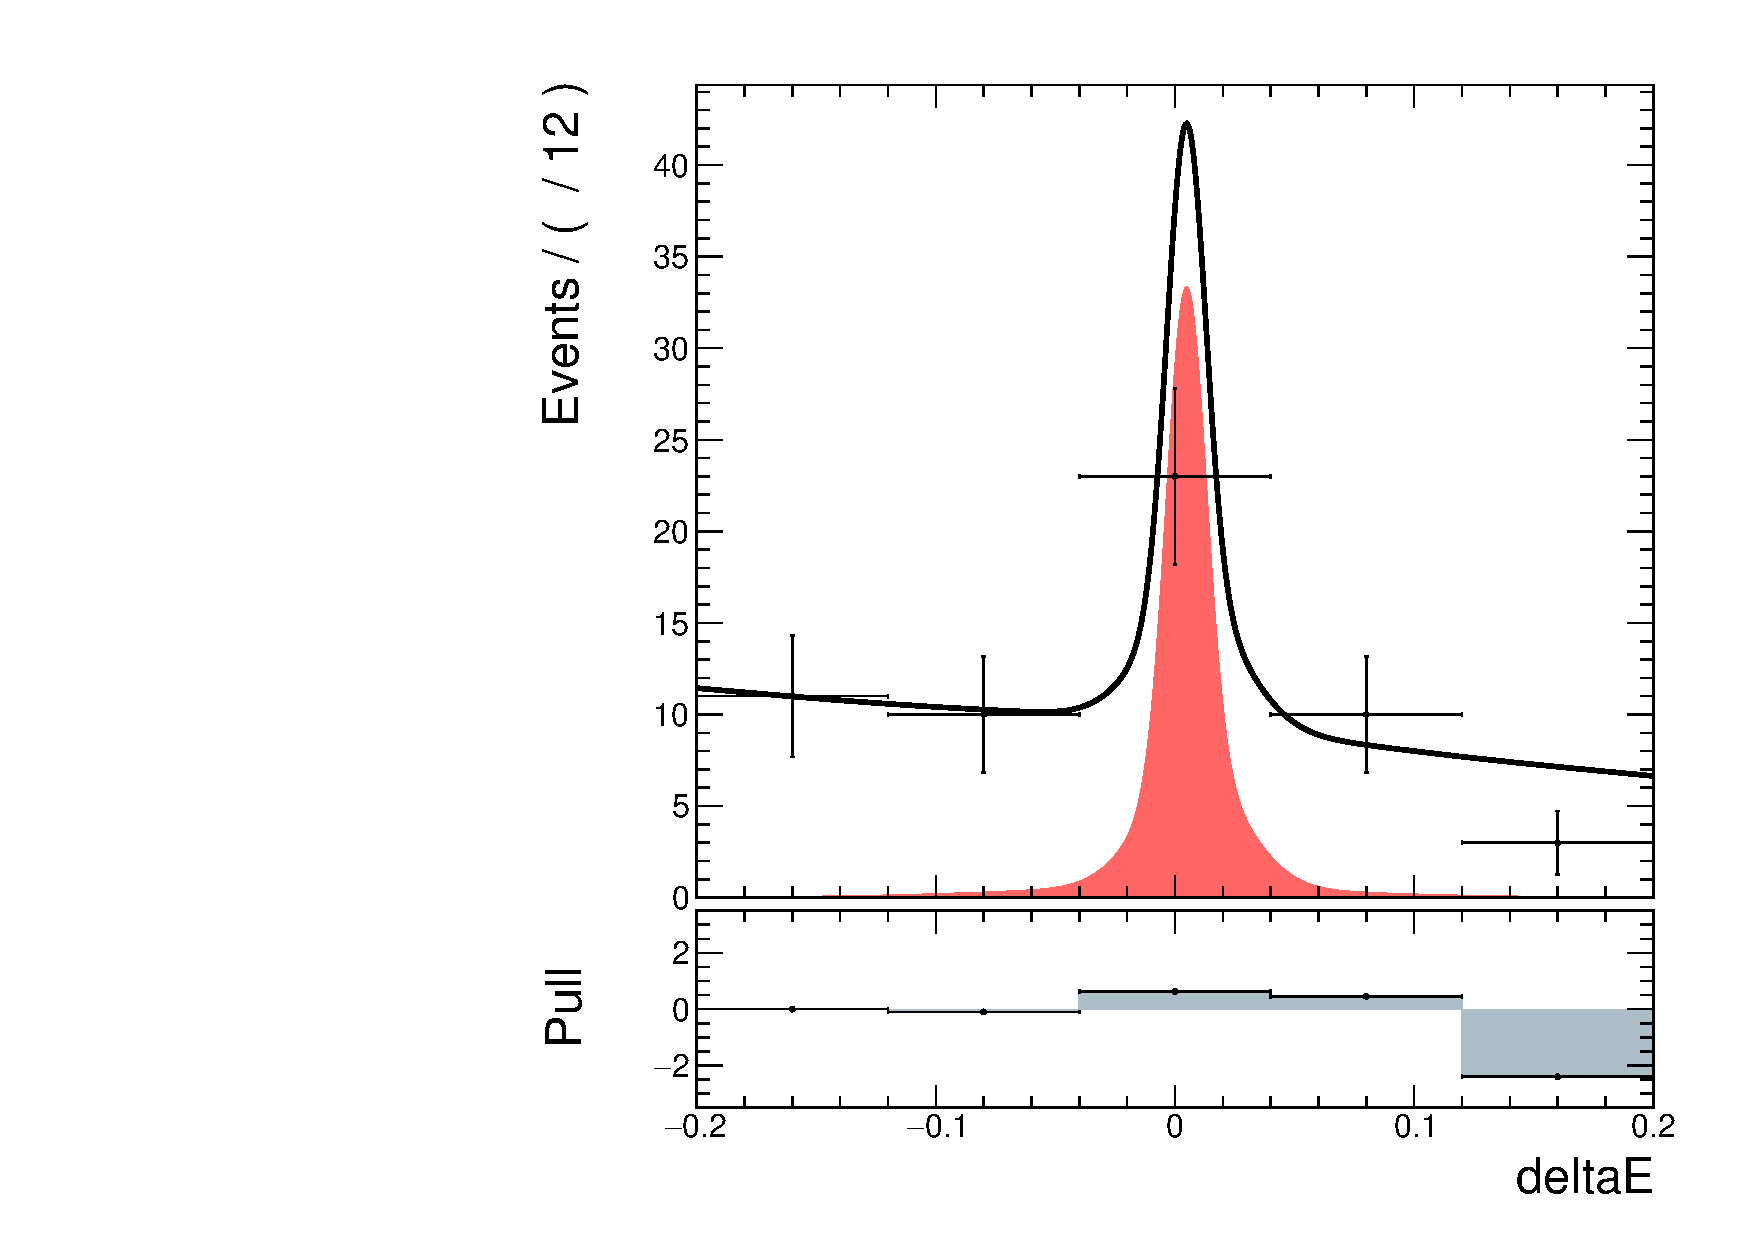
\includegraphics[page=1,height=6cm]{figures/injection_sig_10/ds_gen_deltaE_2D.pdf}
		\caption{signal injected: 10}
	\end{subfigure}
	\begin{subfigure}{0.5\linewidth}
		\includegraphics[page=1,height=6cm]{figures/injection_sig_15/ds_gen_Mbc_2D.pdf}
		\caption{signal injected: 15}
	\end{subfigure}
	\begin{subfigure}{0.5\linewidth}
		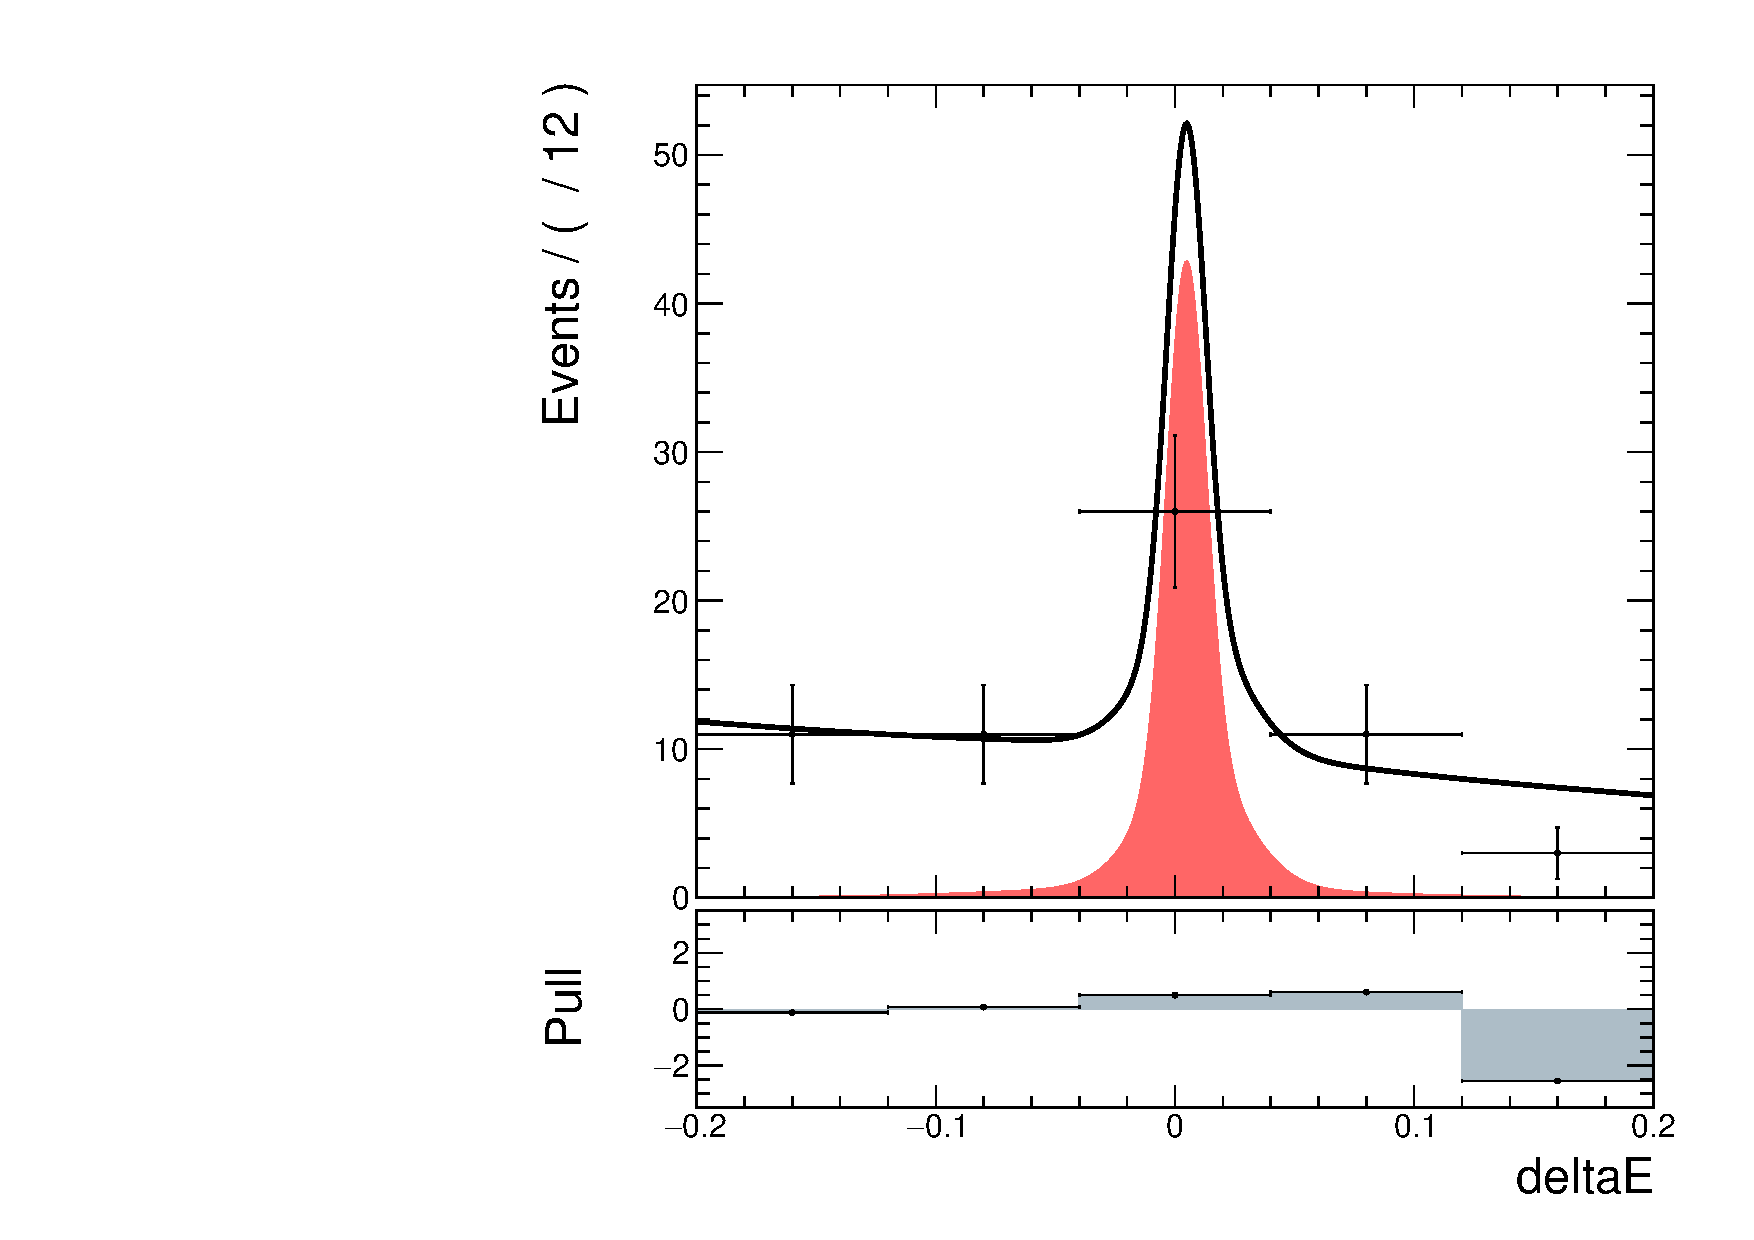
\includegraphics[page=1,height=6cm]{figures/injection_sig_15/ds_gen_deltaE_2D.pdf}
		\caption{signal injected: 15}
	\end{subfigure}
\end{figure}

\begin{figure}[htpb]
	\ContinuedFloat
	\begin{subfigure}{0.5\linewidth}
		\includegraphics[page=1,height=6cm]{figures/injection_sig_20/ds_gen_Mbc_2D.pdf}
		\caption{signal injected: 20}
	\end{subfigure}
	\begin{subfigure}{0.5\linewidth}
		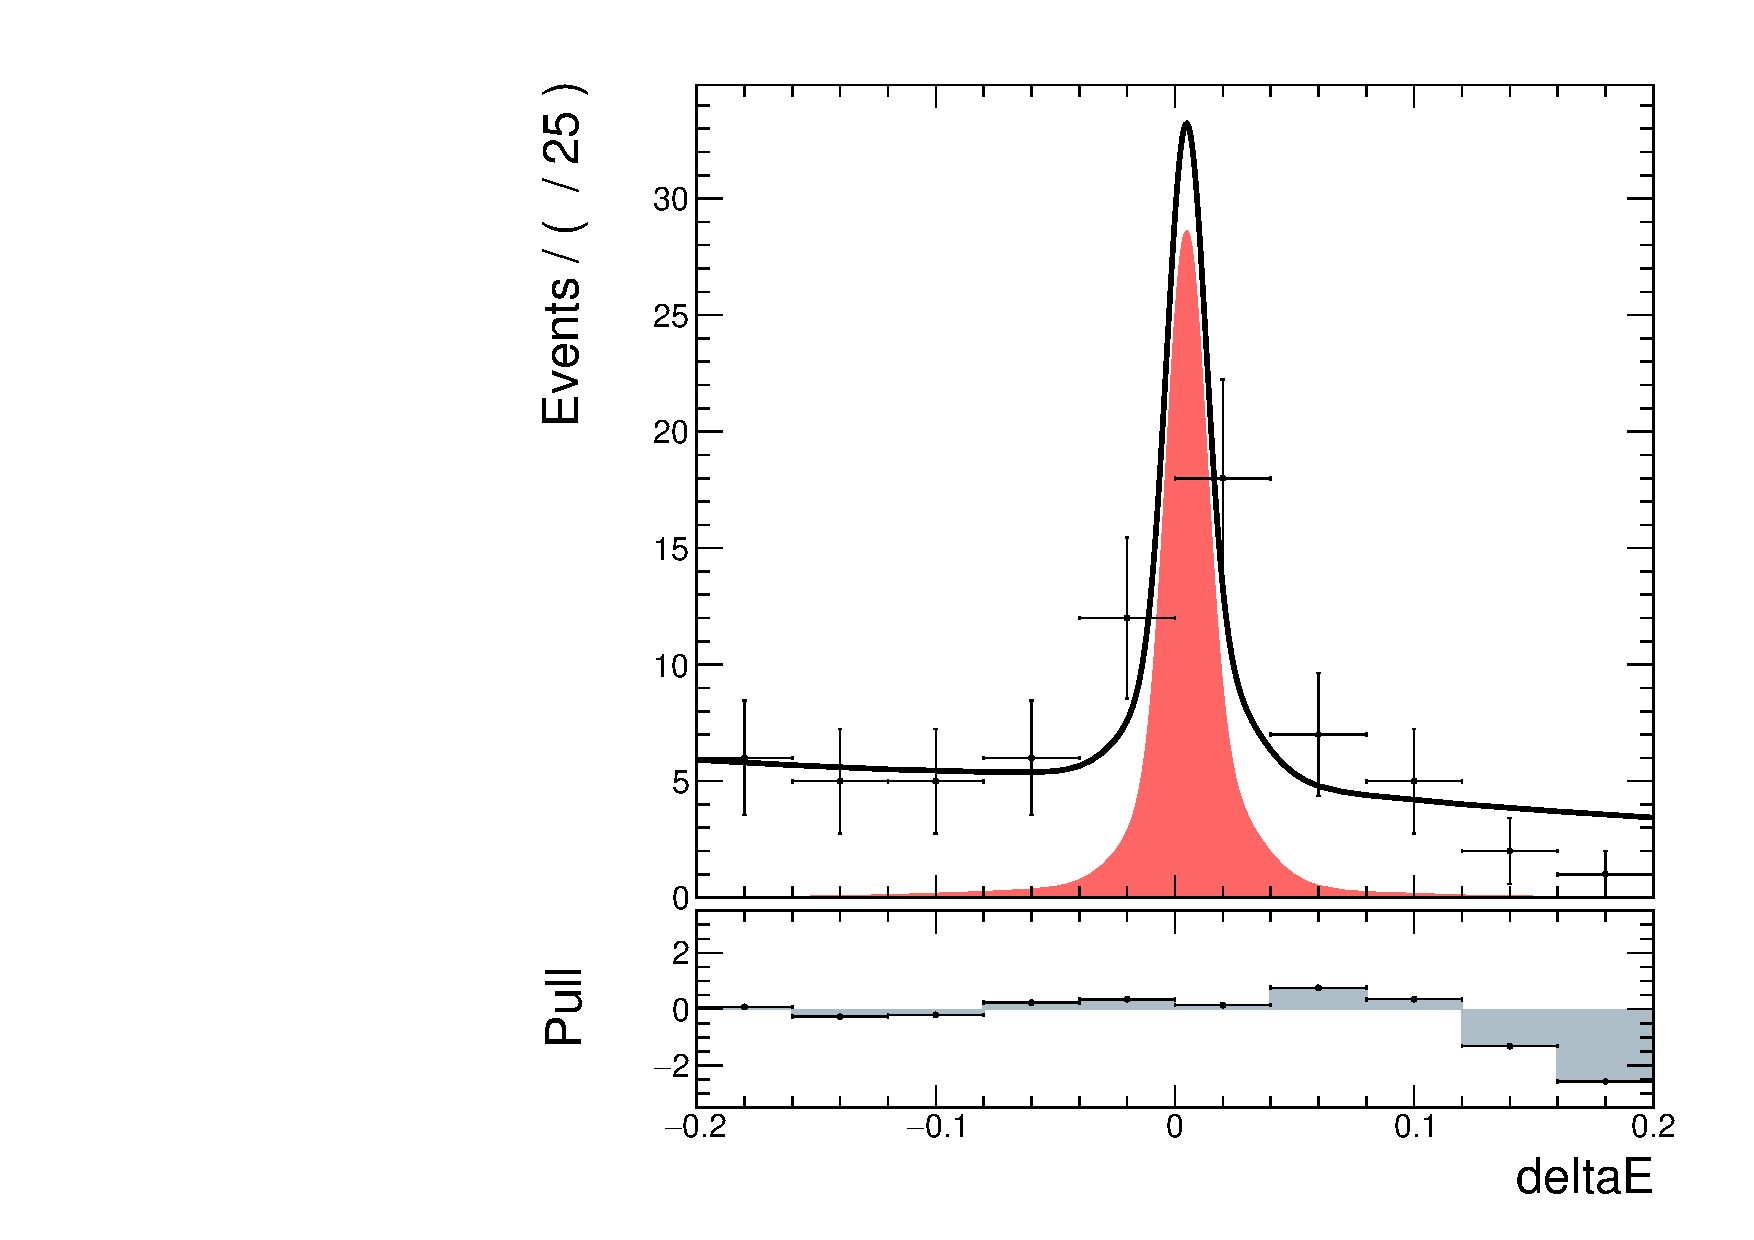
\includegraphics[page=1,height=6cm]{figures/injection_sig_20/ds_gen_deltaE_2D.pdf}
		\caption{signal injected: 20}
	\end{subfigure}
	
	\begin{subfigure}{0.5\linewidth}
		\includegraphics[page=1,height=6cm]{figures/injection_sig_25/ds_gen_Mbc_2D.pdf}
		\caption{signal injected: 25}
	\end{subfigure}
	\begin{subfigure}{0.5\linewidth}
		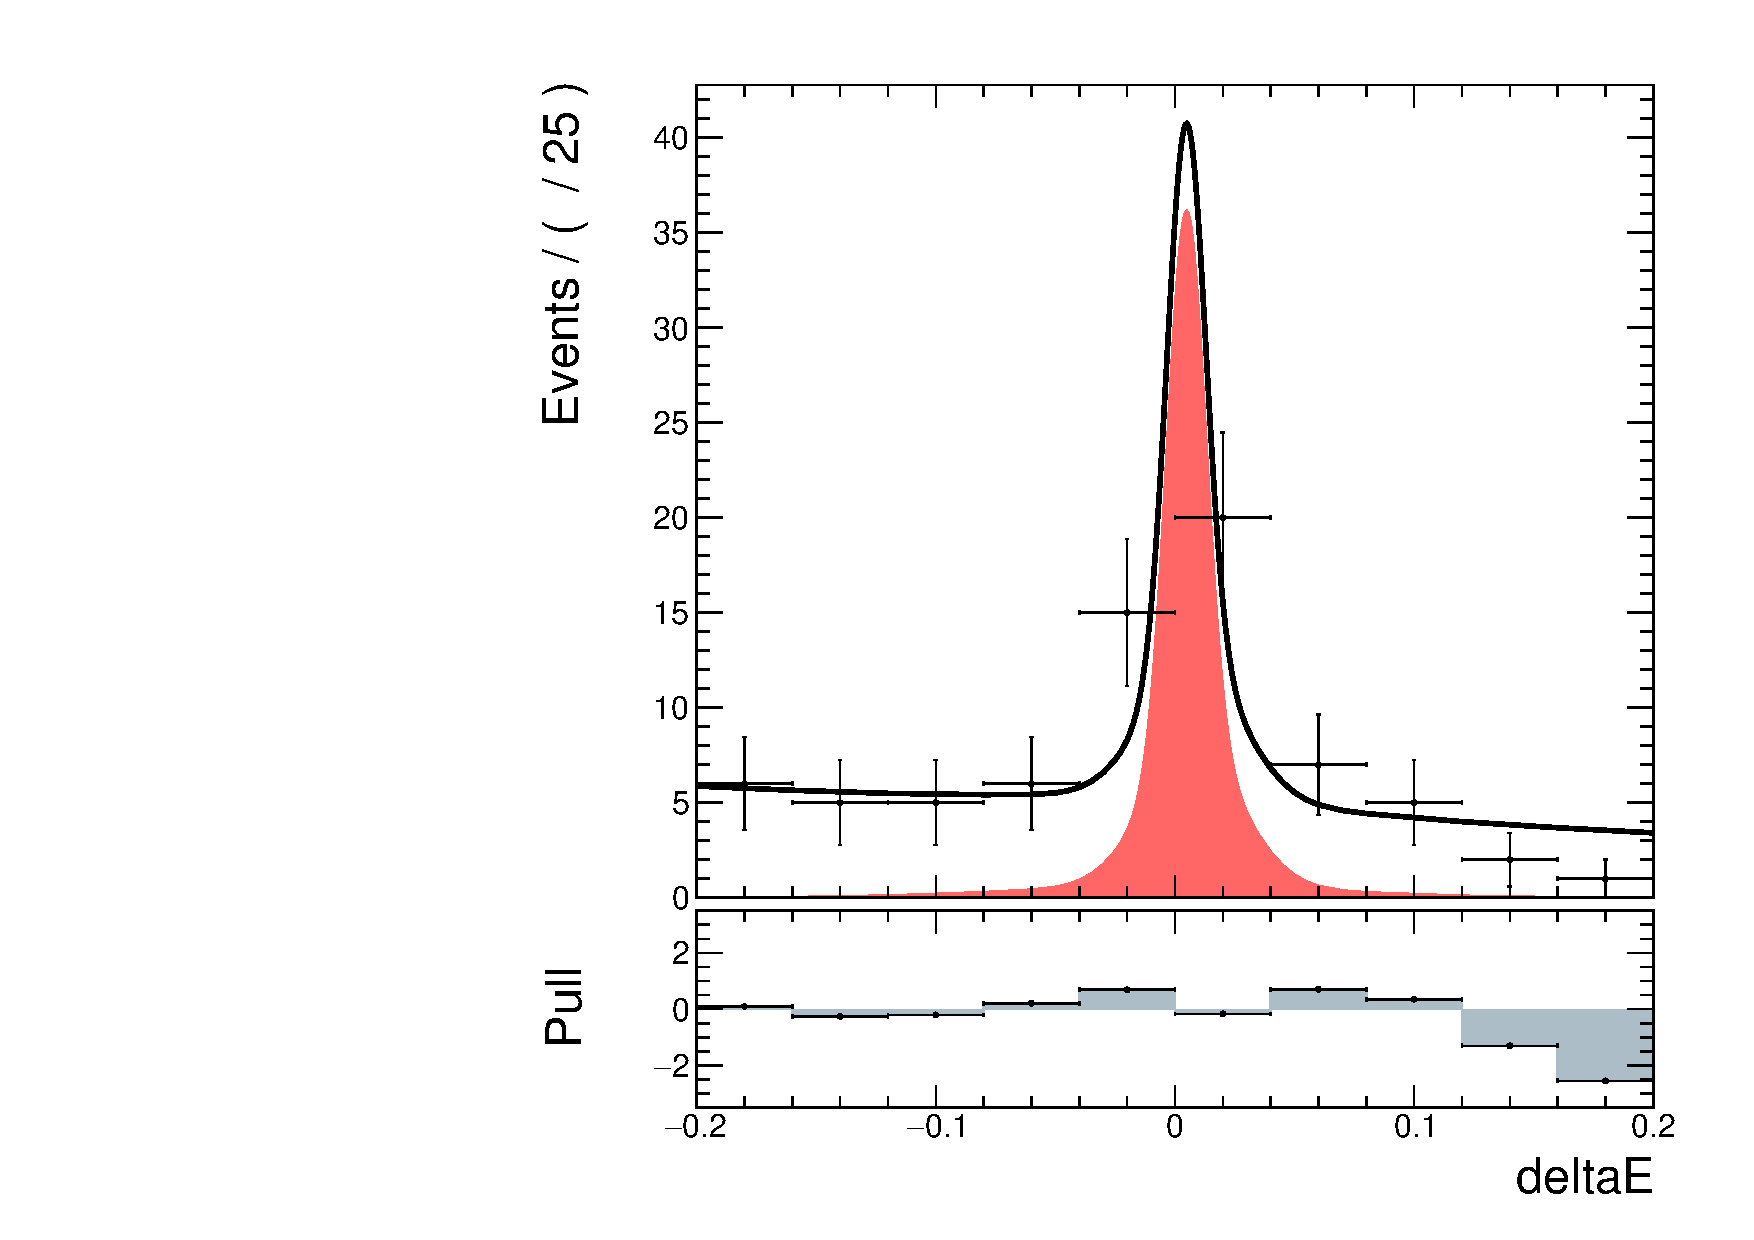
\includegraphics[page=1,height=6cm]{figures/injection_sig_25/ds_gen_deltaE_2D.pdf}
		\caption{signal injected: 25}
	\end{subfigure}
	\begin{subfigure}{0.5\linewidth}
		\includegraphics[page=1,height=6cm]{figures/injection_sig_30/ds_gen_Mbc_2D.pdf}
		\caption{signal injected: 30}
	\end{subfigure}
	\begin{subfigure}{0.5\linewidth}
		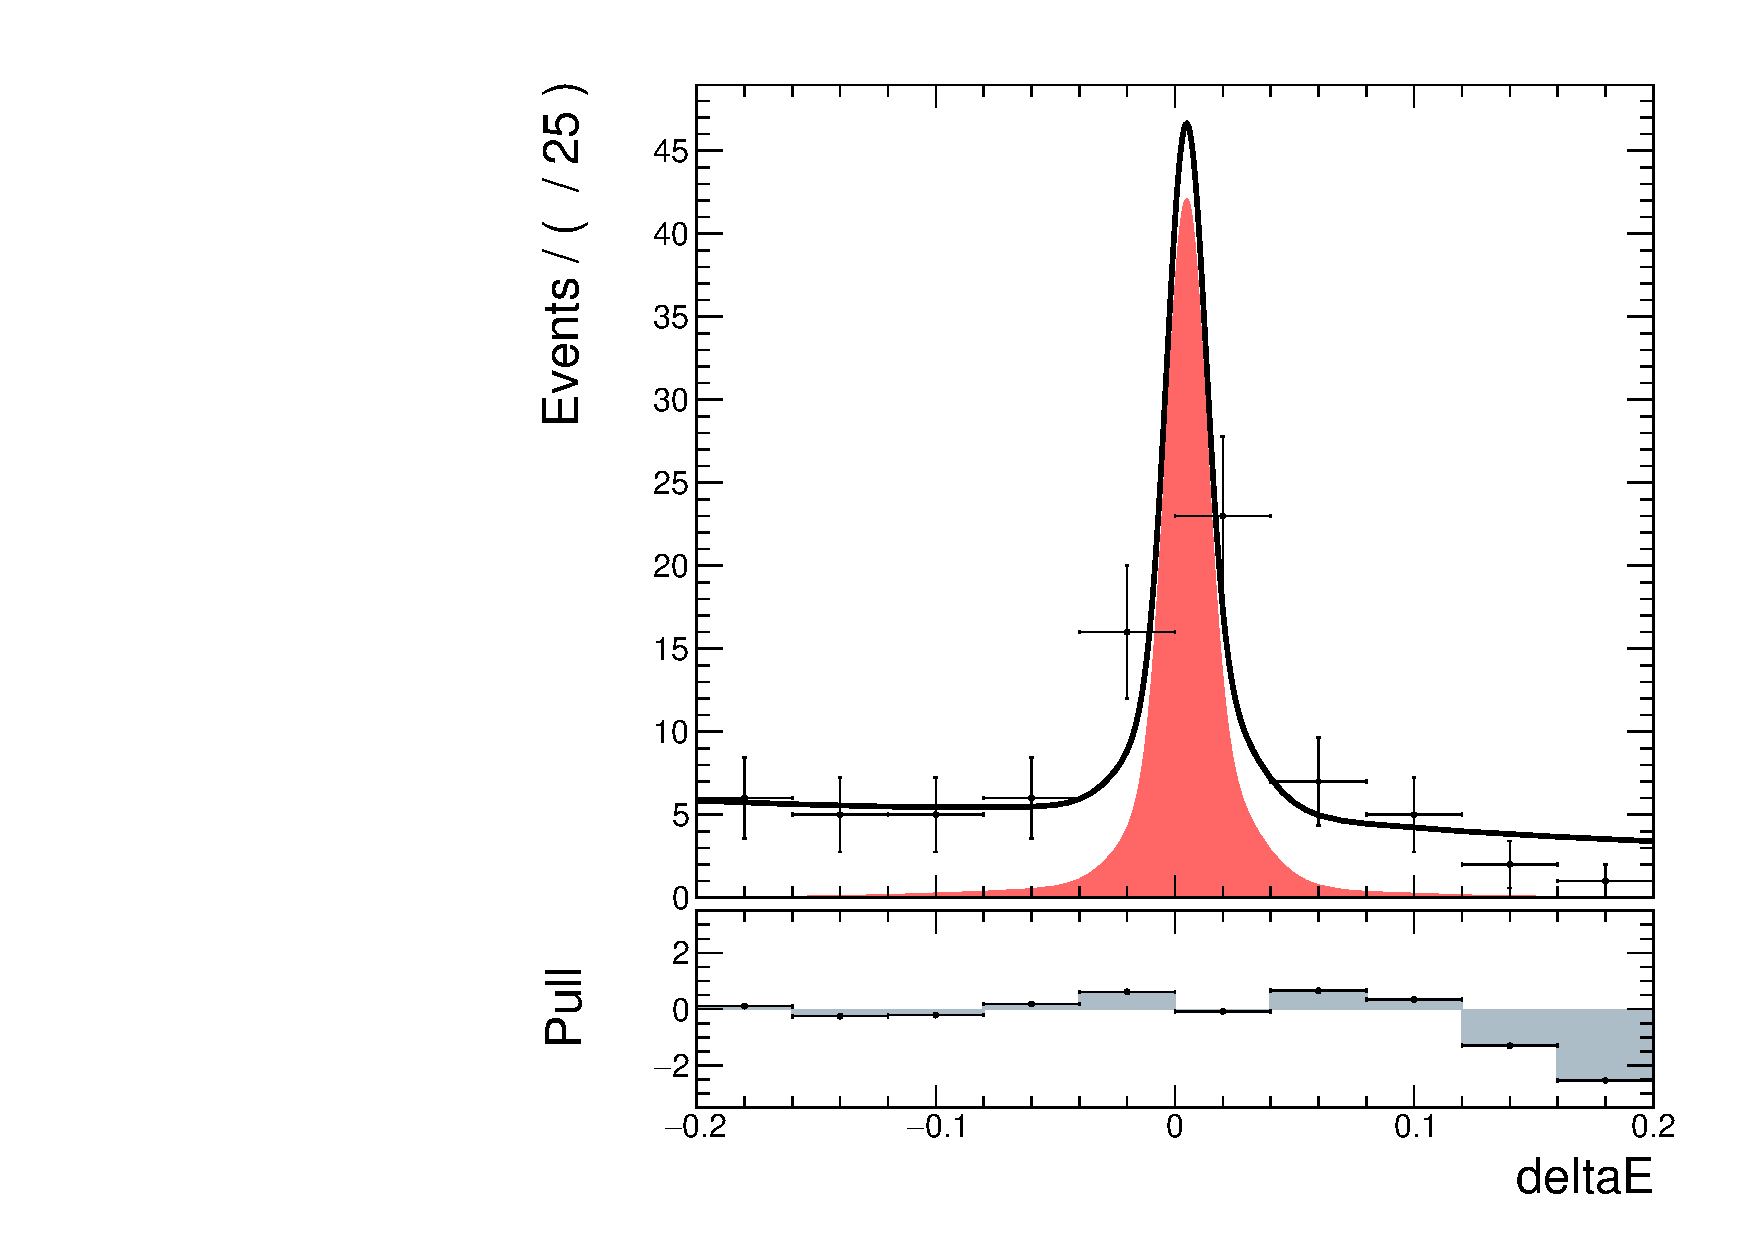
\includegraphics[page=1,height=6cm]{figures/injection_sig_30/ds_gen_deltaE_2D.pdf}
		\caption{signal injected: 30}
	\end{subfigure}
	\caption{The fit results of $M_{bc}$ and $\Delta E$ in signal injection test, where signal events from 5 to 30 with 5 per step are injected with 46 continuum events.}
	\label{fig:injectiontest}
\end{figure}